\chapter{Methods}\label{chapter:method}

{ \color{red}

    about 10-30 pages (rather more I guess)

    \begin{itemize}
        \item (1/3 of thesis)
        \item start with a theoretical approach, describe the developed system/algorithm/method from a high-level point of view,
        \item go ahead in presenting your developments in more detail
        \item make sure to not refer to results section too much. rather leave info out if it cannot explained well without looking at the results
    \end{itemize}
}

\section{Causal Model}
In principle, our analysis combines causal methods for data generation and ground-truth feature attribution. 
The process starts with intervening on a hyperparameter such as the later discussed coupling ratio $\rho$, then training models and finally generating predictions and explanations. 
Within this greater structure, a subprocess generates the images used for training with a structural causal model, taking only $\rho$ as an input. While $\rho$ stays fixed for a single instance of data generation, it is a causal variable in the overarching model. 

\subsection{Data Generating Causal Model}
For the most exact comparison of attribution between a model and its explanation it is imperative to know the ground truth of the training data. A structural causal model (SCM) can define variables and the \textit{independent} mechanisms with which they interact precisely. We want to define an SCM that closely mirrors image generation processes as they happen in realistic scenarios. 
Explicitly using a generating SCM has previously been done to create or test new attribution methods \cite{Parafita2019, Wilming2023,Clark2023, Goyal2019, Reimers2019, Reimers2020}. A few other works evaluating XAI methods with a known ground truth have implicitly used structures akin to an SCM without defining it in causal language \cite{Kim2018, Yang2019,Arras2022}. 

The causal graph and its structural assignments used for our experiment are defined as follows: 
\begin{align}
&G:=\mathcal{N}(0.5,0.02) \notag \\ 
&N_w:=\eta^w &\mathrm{with} \  \eta^w \sim \mathcal{N}(0.5,0.1) && \notag \\ 
&N_s:=\eta^s &\mathrm{with} \  \eta^s \sim \mathcal{N}(0.5,0.1) && \notag \\ 
&N_x:=\eta^x &\mathrm{with} \  \eta^x \sim \mathcal{N}(0,0.05) && \notag \\ 
&W:=\rho * G + (1-\rho)* N_w \notag \\ 
&S:=\rho * G + (1-\rho)* N_s \notag \\ 
& \mathcal{X} = f_{image}(W, S, Z) + N_{x} &
\end{align}

\begin{figure}[H]
    \centering
    \includegraphics[width=0.9\textwidth]{pics/generating_scm.png}
    \caption{Structural causal model for first experiment.
        In the top right corner the distribution of the variables Watermark $W$ and Shape $S$ are plotted against each other to show the effect of $\rho = 0.6$. Note how $\rho$ is not a causal variable but merely a hyperparameter. It determines the degree to which $G$ confounds $W$ and $S$. The other factors $Z$ might also have noise terms, which we do not show explicitly.}
    \label{fig:generating_scm}
\end{figure}

The SCM as seen in \cref{fig:generating_scm} and \cref{eq:scm} serves as a ground truth for our first experiment. It is an additive model using Gaussian distributions for the noise terms. In realistic datasets the generating mechanisms are usually more complex and distributions mostly not exactly Gaussian, one can thus theoretically extract causal directions better because they are identifiable.
Still, identifying causal directions is very hard and not the goal for a neural network in many realistic cases, regardless whether the noise might not be Gaussian and the relations not linear.

The meta-variable $\rho$ adjusts how much information is shared between the true class information (shape), which we name \textit{core feature} following \cite{Singla2022} and the watermark or \textit{spurious feature} through a shared common ancestor named generator $g$. For each model/data combination coupling $\rho$ is fixed, to later enable a comparison between models trained with different coupling ratios. 

The idea of investigating the effect of such a coupling ratio $\rho$ was inspired by Wilming et al. \cite{Wilming2023}, who also used a \textit{signal-to-noise} ratio in their generating model. Instead of a confounding model their learned data instances are colliders of their label and a suppressor variable. The expected explanation importance of this suppressor feature therefore ought to be zero, as long as the collider is not intervened on. We contest this assumption, as it is not clear whether a neural network does not implicitly create interventions on this collider (which is the image), therefore introducing correlation between the parent components. 

A second parameter which we keep fixed for all experiments, determines how frequent the spurious feature is in the data. We set this parameter which could be termed \textit{prevalence} to 0.5, so that just as many images have a watermark as not. It is important to note that this particular SCM is just one of many possible ways to model how spurious features might interact with core features. It attempts to follow the logic of how images are generated or selected in real datasets. Here, it particularly looks at pathways for the generation of \textit{Clever-Hans} or \textit{watermark} features, often present in image datasets \cite{Lapuschkin2019}. As visible in \cref{fig:equivalent_scm} different causal models can produce an equivalent distribution of the two latent factors in question (watermark and shape). One can think of more variations of SCMs which are able to produce the same correlation, so the choice of using the confounder version as in \cref{fig:generating_scm} is mainly due to its ease of implementation. Without assumptions about the generating mechanism, the confounder case is not identifiable, i.e. distinguishable, from $W \rightarrow G \rightarrow S$ and $S \rightarrow G \rightarrow W$ because it is Markov equivalent to those scenarios. 
Although the presented collider case (\cref{fig:generating_scm}\textbf{a}) is theoretically distinguishable from the confounder case (\textbf{b}), one can not hope that a network which only has access to the intervened on (selected) data will recover this. 

The direction of causal links for image classification is highly debatable and shall not be the focus of this work. Whether the selection of the AI researcher reducing costs with free images resulted in classes being polluted with watermarks (\cref{fig:equivalent_scm}\textbf{a}), or whether a scientist marked x-rays with their diagnosis (\cref{fig:equivalent_scm}\textbf{b}) is indistinguishable for ML models. 
Instead, we only want to find to what degree a neural network learns, and attribution method explains the distribution generated by a particular SCM.

To evaluate the results of the current experiment and see how having a different SCM might influence the outcome we will later look at other generating SCMs too (\cref{chapter:results}).

\begin{figure}[H]
    \centering
    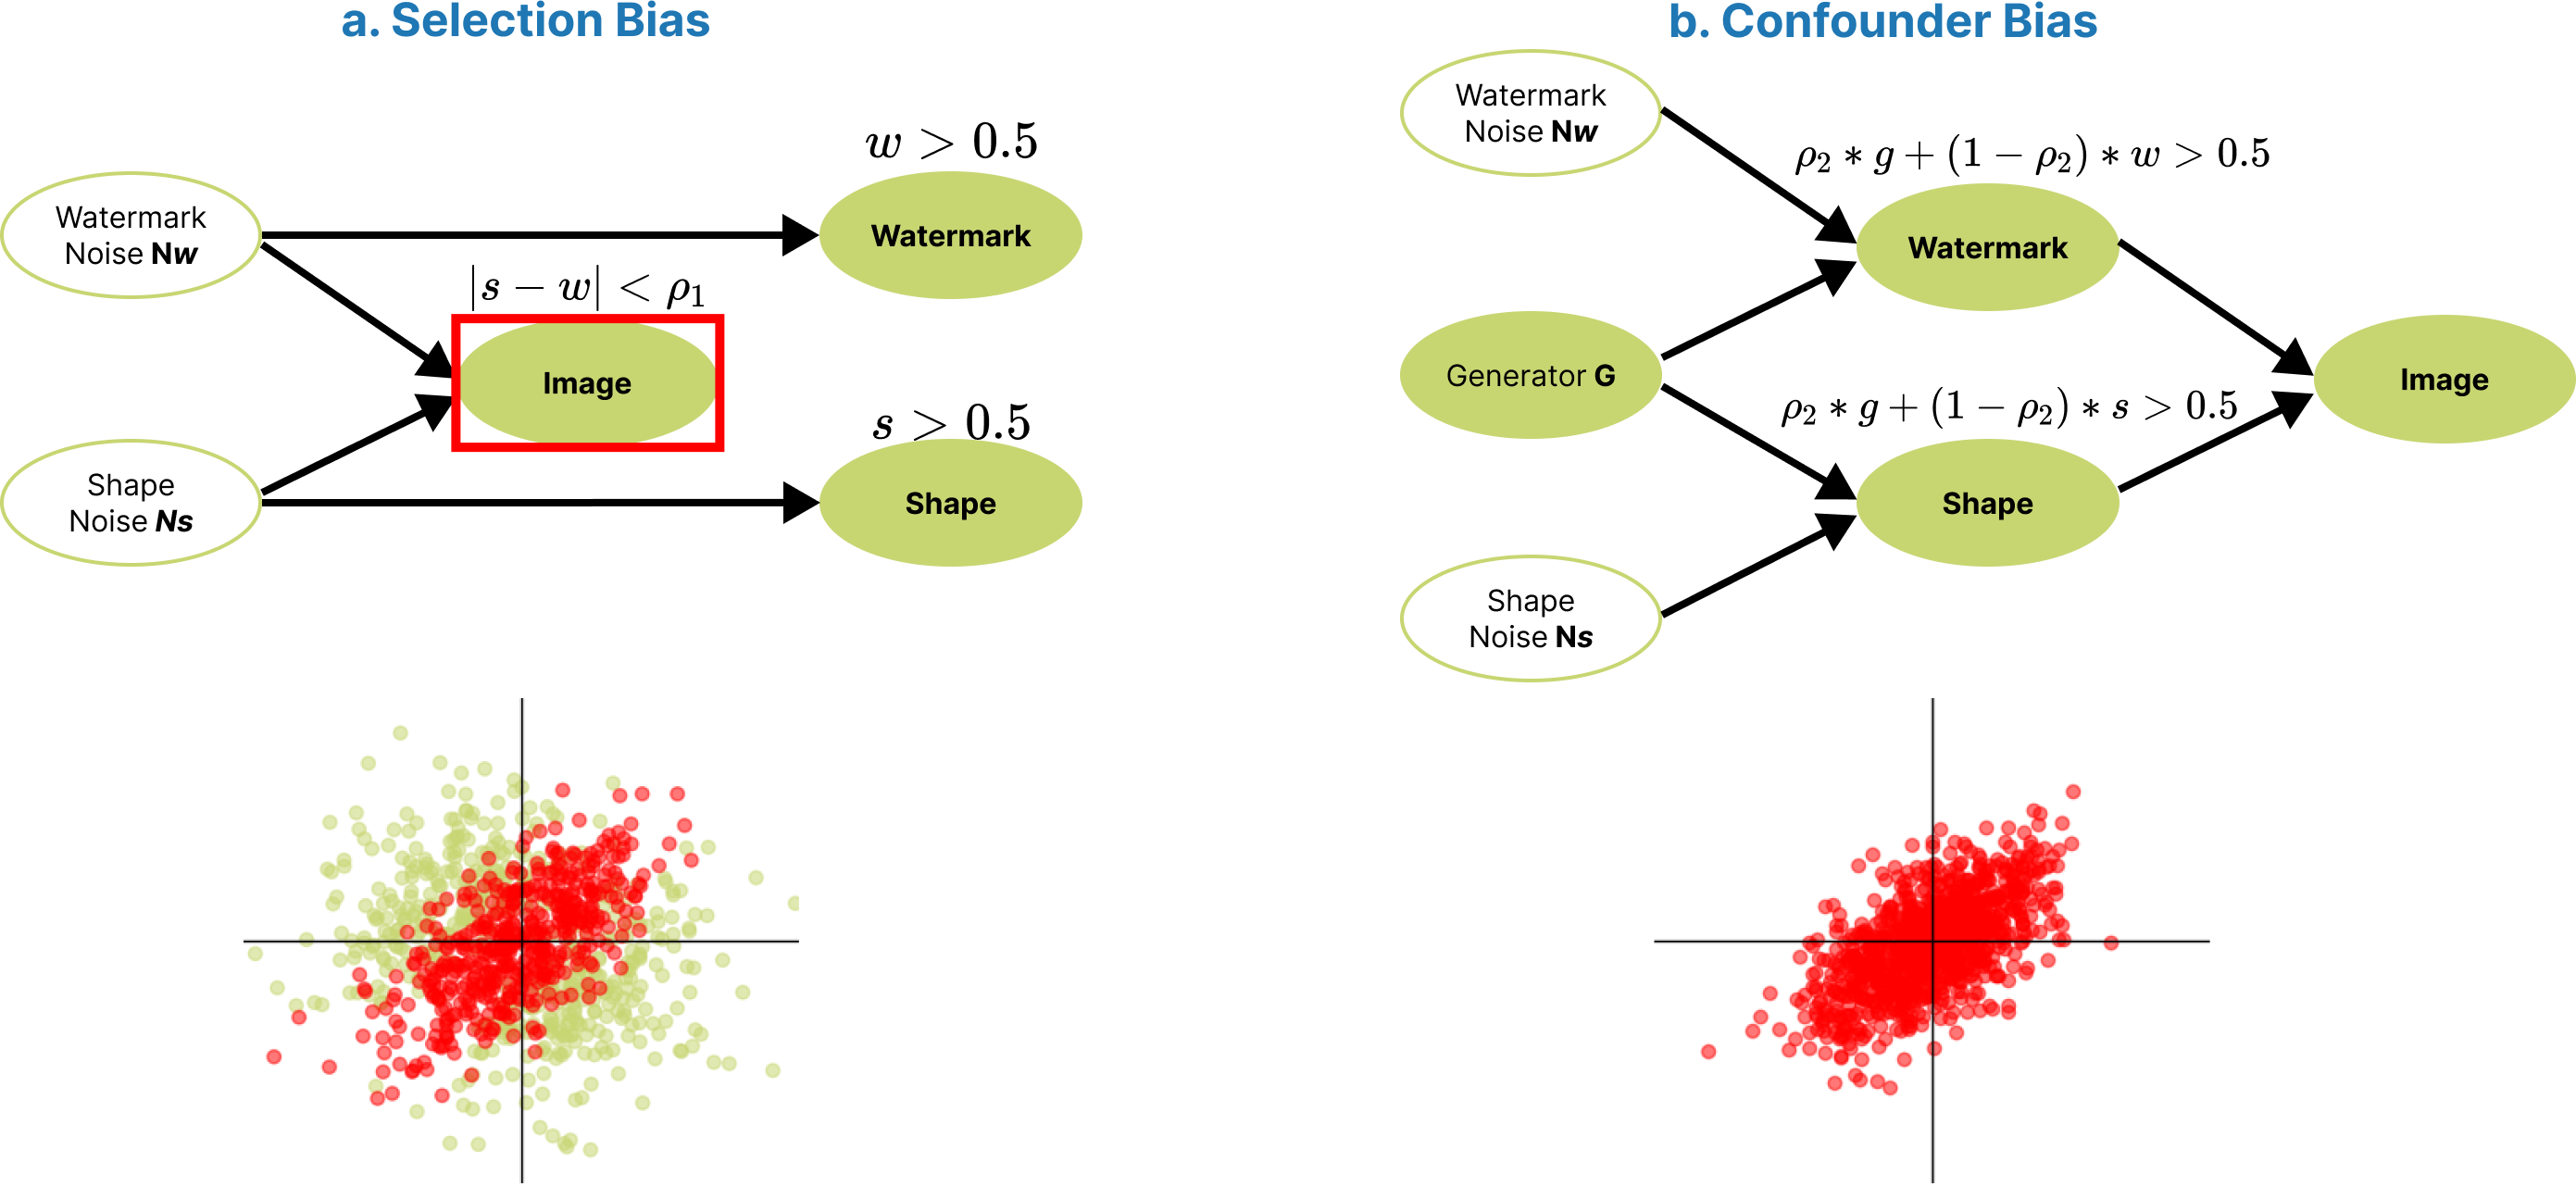
\includegraphics[width=0.8\textwidth]{pics/equivalent_scm.png}
    \caption{SCMs typically found in image datasets.
    \textbf{a.} Selection Bias \textit{(researcher chooses images from free online collection with watermarks)}
    \textbf{b.} Confounder Bias \textit{(e.g. scientist marks positive x-ray scans with sign)}}
    \label{fig:equivalent_scm}
\end{figure}

\subsection{Explanation Generating Model}
The data generation causal model is part of the model which generates predictions and explanations.
This model is defined in a similar way to the \textit{explanation generating process (EGP)} in Karimi et al. \cite{Karimi2023}.
Ratio $\rho$ is a meta-variable of our image generation process in a similar sense to how hyperparameters are defined for the training there. While \cref{fig:generating_scm} depicts the data generating causal model (DGCM) of the training dataset in more detail, \cref{fig:egp} shows how this is embedded into the mechanism of generating explanations. 

\begin{figure}[H]
    \centering
    \tikzset{%
        neuron/.style={
                circle,
                draw,
                minimum size=8mm
            }
    }
    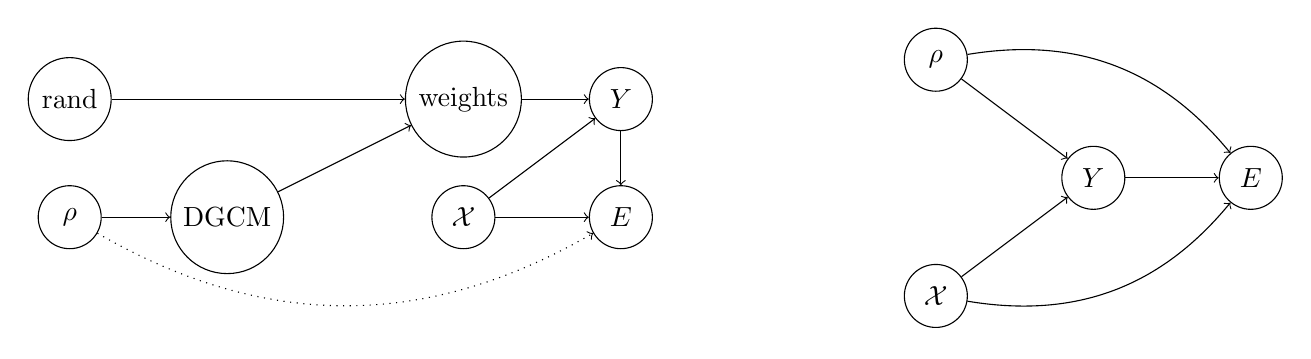
\begin{tikzpicture}[every node/.style={ draw, minimum size=8mm, align=center},]

    % generating model:
        \node [neuron]  (r) at (0.0,1) {$\rho$};
        \node [neuron]  (rs) at (0,2.5) {rand};
        \node [neuron]  (scm) at (2,1) {DGCM};
        \node [neuron]  (ws) at (5,2.5) {weights};
        \node [neuron]  (x) at (5,1) {$\mathcal{X}$};
        \node [neuron]  (p) at (7,2.5) {$Y$};
        \node [neuron]  (e) at (7,1) {$E$};

        \draw[->] (r) -- (scm);
        \draw[->] (rs) -- (ws);
        \draw[->] (scm) to (ws);
        \draw[->] (ws) -- (p);
        \draw[->] (x) -- (p);
        \draw[->] (x) -- (e);
        \draw[->] (p) -- (e);
        \draw[->, bend right=30, dotted] (r) to (e);
        
    % simplified causal model:
        \node [neuron]  (r) at (11,3) {$\rho$};
        \node [neuron]  (x) at (11,0) {$\mathcal{X}$};
        \node [neuron]  (p) at (13,1.5) {$Y$};
        \node [neuron]  (e) at (15,1.5) {$E$};

        \draw[->] (r) -- (p);
        \draw[->] (x) -- (p);
        \draw[->, bend right=30] (x) to (e);
        \draw[->] (p) -- (e);
        \draw[->, bend left=30] (r) to (e);
    \end{tikzpicture}
    \caption{Explanation Generation Process \textit{EGP} (left), Simplified Causal Model (right)}
    \label{fig:egp}
\end{figure}

\subsection{Watermark Benchmark Dataset W-dSprites}\label{section:causal_model}
Although this thesis is not the first work to use a toy dataset with known generating factors to evaluate attribution methods, we aim to find a new dataset which is as simple as possible and yet mirrors the main workings of a realistic computer vision problem. For this we adapted the dSprites dataset \cite{dsprites17} by adding small watermarks in the shape of '\textit{w}'s to some images. The dSprites dataset was originally constructed as a means for testing the degree of disentanglement a machine learning model has achieved. It contains images with rectangles, ellipses or hearts in varying positions, scales and rotations. To simplify the task more we only use the rectangle and ellipse class for our experiment. Another motive is that in a binary classification task positive and negative relevance might be used in varying strategies for prediction. In theory this could make the class-insensitivity studied by Sixt et al. \cite{Sixt2020} visible or counteract it. Further details can be found in the appendix \cref{appendix:dsprites}.

\begin{figure}[H]
    \centering
    \includegraphics[width=0.6\textwidth]{pics/dsprites_examples.png}
    \caption{First row: images from the original dSprites dataset, second row: images from the W-dSprites dataset with small \textit{w} as a watermark on some images in random positions at the edge of the image and Gaussian noise added.}
    \label{fig:dsprites_examples}
\end{figure}

\section{Generating Explanations with Concept Relevance Propagation}
The previously described causal framework can be applied to a multitude of explanation methods as it is principally model- and method-agnostic. However we limit our analysis to CRP, its predecessor LRP and interpretation techniques constructed with CRP.
Producing explanations using concept relevance propagation requires decisions on the backpropagation rule(s), on the conditioning sets and potentially further hyperparameters. 
We follow the recommendations or default settings of CRP's authors \cite{Achtibat2022, Achtibat2023} and best practices \cite{Kohlbrenner2020} as closely as possible.
For the backpropagation we apply the $LRP_{\varepsilon -z^+- b^-}$ - rule as recommended by \cite{Kohlbrenner2020}. Due to the simplicity of our CNN model no more model canonization steps need to be applied. See \cref{appendix:lrprules} for further technical details. 

\begin{figure}
    \centering
    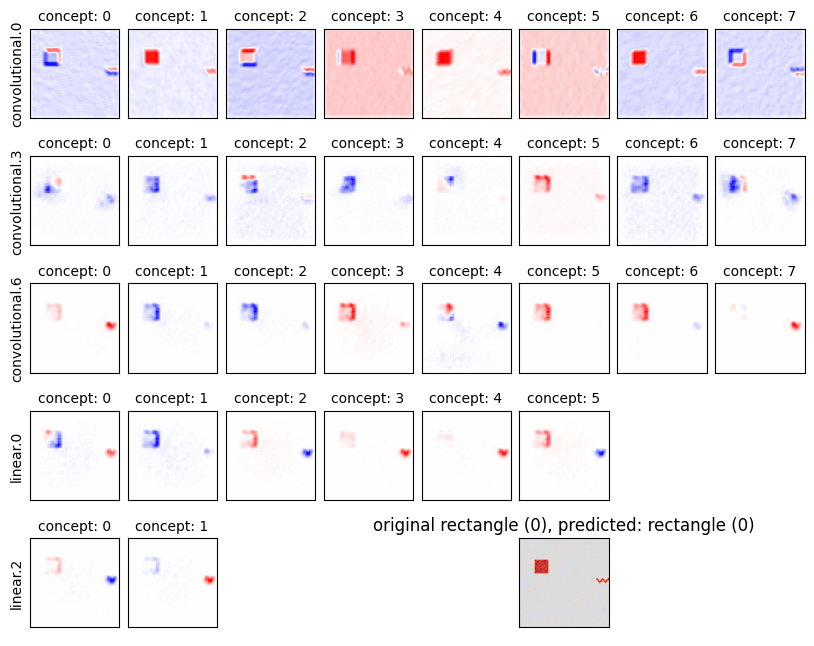
\includegraphics[width=0.8\textwidth]{thesis_latex_template/pics/conditional_heatmaps.png}
    \caption{Concept-conditional heatmaps for one example image. Note the Sobel-filter-like attributions in earlier layers and the more combined attributions of watermark and shape in later layers.}
    \label{fig:cc_heatmaps}
\end{figure}

Principally, neurons in every layer of a model can be conditioned on using the CRP-approach. However, the resulting attribution maps are not necessarily depicting disentangled and abstract enough concepts. When looking at a \textit{concept-conditional} attribution maps from the earlier layers, one will likely see low-level features. In the later fully connected layers before the output the potentially disentangled concepts might get mixed together again for the final decision. In \cref{fig:cc_heatmaps} an example shows the tendency from trivial to abstract \textit{concepts}. 
According to \cite{Dreyer2023a, Zeiler2013} the last convolutional layer is ``most likely representing disentangled representation''. For comparison we investigate both the last convolutional (layer 3) and the first fully connected layer (layer 4) of the 5 total layers. It is not entirely clear whether the extremely small size of our model hinders a transfer of the results to realistic scenarios. Yet training significantly larger models would have been too computationally expensive for this approach. \\

In the following we will reiterate the steps necessary to produce multiple types of explanations with CRP:

\subsubsection{Concept-Conditional Attribution Maps and Relevance for Prediction}
The concept-conditional backpropagation rule described in \cref{section:crp_background} can be applied to arbitrary sets of neurons $\theta$. In our scenario we create class-specific attribution maps conditioned on each neuron in the selected layer (3 or 4). For this we use the output for the predicted class as the initialization for relevance, keep all other layers untouched and then mask out the other neurons relevance in the layer $\ell$. 
\begin{equation}
    R_{i}^{\ell}(\mathrm{x} |\theta_{\ell}=\{i\}) 
\end{equation}
Backpropagating all the way to the input yields an attribution map $R_i^{\ell}$, however the relevance $r_i$ assigned to the neuron in question from previous layers can be used as an approximation of its overall importance for the prediction.

\begin{itemize}
    \item should I keep class the same or change per instance?
    \item Should I really do everything both for last convolutional and first fully-connected layer?
\end{itemize}

{\color{gray} \subsubsection{Relevance Maximization}
To arrive at reference sets of the neurons in our selected layer, relevance maximization finds images that maximize concept-conditional relevance. As mentioned by \cite{Achtibat2022} using the whole dataset might make the selected images too similar to each other. Hence we compute the maximization for a subset of 1000 images to enforce more variance. Importantly, the sample we select from does not have the association between $S$ and $W$, meaning that watermarks are equally likely to occur on rectangle as on ellipse images. 
The implementation provided by CRPs authors produces sets of 40 images for each neuron in each layer. 

\subsubsection{Perceptive Field}
Information on the concentration of the relevance within the images selected for each concept can be gained by applying concept localization. Following the approach of \cite{Yeh2020} and using tools from the existing LRP toolset \cite{Anders2023} Achtibat et al. visualize only the part of the selected images that contributed to the neurons activation. 
The implementation of this and all previously described methods is made accessible by CRPs authors at \url{https://github.com/rachtibat/zennit-crp}.
}


\section{Data Ground Truth Correlation $m_0$}
The goal of this analysis it to gather knowledge on how a known coupling ratio of two features interacts with their true importance to the model and their explained importance. 
Measure $m_0 = \rho$ is the correlation between the shape and watermark feature in our data generating model. When $\rho$ is 0, the features are not associated at all, when it is 1 they correlate perfectly. Conceived as a \textit{signal-to-noise} ratio between the correlated and uncorrelated parts of $S$ and $W$, it can directly be used as a measure of comparison. However the data generating process introduces some noise and it might be more interesting to look at the mutual information of the features in the generated data distribution as a ground-truth. 
Generally, we do not want and neither expect the model to perfectly reconstruct $\rho$. After all, the strength of neural networks presumably lies in recovering the truly important feature even when highly correlated features are present. Though some research expects explanations to give insight into the distributions of the training data to better understand how biases might occur, even if a model has apparently learned to ignore spurious features \cite{Kindermans2017}. 

\begin{figure}
    \centering
    \includegraphics[width=0.5\textwidth]{thesis_latex_template/pics/m0_options.png}
    \caption{$\rho$ plotted against other possible ways to measure ground truth data importance/ correlation of $w$ and $s$}
    \label{fig:finding_rho}
\end{figure}

\section{Establishing a Ground-Truth Model Feature Importance $m_1$}\label{section:gt_measure}
In contrast to realistic application scenarios our causal framework enables us to establish the ground truth importance of features for a trained model. Similar to recent work on causal attribution \cite{Parafita2019,Reimers2020,Karimi2023} the causal effect of an intervention upstream on the output of a model can be estimated in the following way:
\begin{center}
Average Causal Effect of latent factor $W$ on output $Y$ \\
\begin{equation}
\displaystyle ACE = \mathbb{E} [ Y \ | \ do(W=1) ] - \mathbb{E} [ Y \ | \ do(W=0) ] 
\end{equation}
\end{center}
The intervention on a given latent factor is straight-forward here, as our factors of interest are both binary variables (watermark and shape). Due to our knowledge of the ground truth we can just feed one image with the watermark and the same image without it through the neural network. Thereby achieving a perfect intervention on our latent factor.  
However it is not naturally clear how to define the output of a model. One can either measure the average causal effect on the output layers' logits, which change in a continuous fashion, or the effect on the binary prediction. In our example this would be equivalent to the percentage of images for which the prediction flips, when the factor is flipped. 
To account for the unknown effects of the random initialization of model weights and biases on the usage of either feature, we average each measure over multiple predefined random seeds. 

\subsection{Mean Logit Change}
For the W-dSprites binary classification task, the output vector consists of 2 values $y_0$ and $y_1$. The model predicts \textit{rectangle} when $y_0 > y_1$ and \textit{ellipse} otherwise. To compute the mean logit change when intervening on our watermark spurious feature $x$, we take a sufficient amount of samples $\mathcal{X}$ from our dataset and feed them through the model. When $W=1$ the images additionally contain a watermark, when $W=0$ not. 

In \cite{Sixt2022a} paper: "median of the absolute change in logit values"

The Mean Logit Change is computed like this:
\begin{equation}
\displaystyle 
MLC = \sqrt{(\vec{y}_{\mathrm{x}, W=1}- \vec{y}_{\mathrm{x}, W=0})^2}
\end{equation}

\subsection{Prediction Flip}
Computing the Prediction Flip follows mostly the same approach as the mean logit change. The only difference is that instead of computing the average effect of the continuous multivariate output vector $\vec{y}$ we consider the prediction to be the binary class variable $y$ which is 0 for rectangle and 1 for ellipse predictions. 

We expect this variant of the prediction variable to be less sensitive to the spurious watermark feature $W$. The reason being, that while the continuous output (i.e. \textit{confidence}) might already be affected by the spurious feature for weaker biases, the prediction will only flip once the spurious feature becomes more important than the core feature. 

\begin{equation}
\displaystyle 
PF =\frac{1}{|\mathcal{X}|} \sum_{\mathrm{x} \in \mathcal{X}} |y_{\mathrm{x}, W=1} - y_{\mathrm{x}, W=0} |
\end{equation}

\subsection{Coefficient of Determination $R^2$}
should I add this as a ground-truth measure too? others have done so before

\section{CRP Explanation Importance $m_2$}\label{section:measure}
Our goal is to compare the causal effect of an upstream intervention on the true feature importance and then the explained feature importance. After having defined how to measure the models true feature importance, we need to repeat the process for the explanation produced by CRP. It is not well known how humans perceive changes in an explanation and there is no agreed upon scale of importance, so we believe it is best to construct multiple measures to test against each other. {\color{gray} Additionally, the authors of CRP introduce multiple interpretation techniques using this method which potentially enable better human understanding. }Most of the proposed metrics are derived from existing work on evaluating feature importance in XAI \cite{Arras2022} \\

Each candidate should be a variation of measuring the effect of intervening on $W$ on an explanation:
\begin{center}
Average Causal Effect of latent factor $W$ on explanation $e$: \\
\begin{equation}
\displaystyle ACE = \mathbb{E} [e \ | \ do(W=1) ] - \mathbb{E} [ e \ | \ do(W=0) ]
\end{equation}
\end{center}
The core question is, how much of the influence on the explanation of changing $\rho$ goes through our prediction. A perfect explanation assigns just as much importance to a feature as the model. This is one way to describe the fidelity of the explanation to the model. The proposed measures however incorporate other notions of goodness applied for XAI such as \textit{intelligibility, complexity} and \textit{user-friendliness}. \\

The measures introduced in the following are roughly ordered from measures being most true to the numerical effect of intervention to measures reducing the complexity of an explanation. Although human perception is not part of our evaluation, aiming for less complex explanations seems to be more in line with a \textit{good} explanation. While the first measure would require the user to compare multiple heatmaps pixel-wise to understand the effect, later metrics use only one pixel or a reduced (hopefully more human-understandable) concept. 

Many related works remove negative relevances in attribution maps to enable comparison with purely positive methods and avoid cancelling-out effects. We believe, however, that a spurious feature can be negatively as well as positively attributed for a model to be biased. Therefore the measures we introduce mostly equally incorporate both the magnitude of the positive and negative relevance. 

\subsection{Mean Attribution Change}
The likely most straight-forward way to calculate explanation importance for neurons in a layer using CRP is to measure the average causal effect of an intervention on the attributions directly. This approach tries to emulate the \textit{mean logit change} of the prediction for the concept-based explanation. In a given layer $\ell \in L$, computing conditional attributions for each of the $|\ell|$ neurons results in $|\ell|$ concept-conditional heatmaps. Also, the total relevance of each those neurons for the overall prediction can be computed using CRP.

We compute the attribution map and its total relevance with the CRP method the following way:
\begin{align*}
& R_i^{\ell}(\mathrm{x}) = R(\mathrm{x} | \theta=\{i, y\}) \\
& r_i(\mathrm{x}) = R(i | \theta=\{y\}) \\
\end{align*}

The causal effect of intervening on the spurious watermark feature on one neuron is then the difference between its attribution map of one image with a watermark and the same image without a watermark. For an approximation of the total difference for a model, one can also weigh each neurons attribution map difference with the neurons relevance for the prediction. If a model has learned the watermark as a distinct concept, but is not using it, the relevance of this concept should be low. \\

To look at the difference in attribution multiple distance metrics could be applied. We compare three types of dissimilarity between two heatmaps (i.e. 2-dimensional pixel maps). Firstly, we look at the mean absolute pixel-wise difference. The Euclidean distance for two images seems the second natural approach. To make the results comparable we normalize each attribution map, which makes the ordering of this metric equal to the ordering if one where to take the \textit{cosine distance}.
Lastly, we compare these to the kernelized treatment effect which Karimi et al. also use for their experiment \cite{Karimi2023}. \\ 



\begin{align}
& ||R(x) - R(x')|| \notag \\
& \sim \sum_{p \in P_x} |R(x)_p - R(x')_p| \\
& \sim \sqrt{\sum_{p \in P_x}\left( \frac{R(x)_p}{|R(x)|} - \frac{R(x')_p}{|R(x')|} \right) ^2} \\
& \sim k(R(x) ,R(x) ) + 2 k(R(x) ,R(x') ) + k(R(x') ,R(x') )  
\end{align}

Once a distance metric is chosen, we need to aggregate results over the neurons in a layer.

\begin{align}
& \frac{1}{|M_\rho|\cdot |\mathcal{X}| \cdot |\ell| }\sum_{m}^{M_{\rho}} \sum_{\mathrm{x,x'}}^{\mathcal{X}} \sum_{i}^{\ell} || R_{m,i}(x) - R_{m,i}(x') || \cdot |r_{m,i}(x) |
\end{align}

While the absolute difference and kernel metrics keep the overall relevance intact, normalizing the euclidean distances means that we are losing this information. Therefore the neuron-wise results of the latter need to be weighted by their original relevance $r$ for the prediction to have a meaningful result. 
We create a (weighted) sum over the neurons $i$ for each sample image $x$ ($x'$ with watermark). 
We again average this over all images $\mathcal{X}$ for the differently initialized models $M_\rho$ for each value of $\rho$.

Which measures did I actually compute now?:
\begin{itemize}
    \item m1, mean logit change with euclidean distances, normed after computing all
    \item m1, mean logit change, normed by max absolute per vector
    \item m1, prediction flip
    \item m2, mean attribution change, absolute distance per pixel
    \item m2, mean attribution change, normalized euclidean distance
    \item m2, rma, mean absolute difference per neuron
    \item m2, rra, mean absolute difference per neuron
    \item m2, rra, mean absolute difference per neuron, weighted by relevance
    \item m2, rra, euclidean distance
    \item m2, pg, mean absolute difference weighted by relevance
    \item m2, kernel (linear) like Karimi
\end{itemize}

Although this weighted difference is constructed to measure the causal effect of intervention on the explanation as closely as possible, it ignores the core idea of CRP's potential usefulness. If adding or removing a watermark has a significant effect on some background pixels far away from it, this is not in line with desirable properties of a good explanation such as interpretability or even fidelity to the ground truth importance. It is likely that through the coupling of watermark and shape in our experiment, the changes of relevance do not only affect the watermark region itself but at least the shapes importance too. 
Another potential downfall for human intuition is the way more localized concepts are attributed in comparison to more global or wide-spread concepts. Achtibat et al. \cite{Achtibat2022} show an example where the eye of a dog wrongly seems to be more important than its fur in a general attribution map, because it is concentrated on a smaller region. A similar thing can potentially happen with our experiments watermark, as it fills a small region in comparison to the larger shape feature. 

For completeness of comparison we compute the same measure for the LRP importance. In this case we just take the average difference when the watermark feature $W$ is intervened on for the heatmap computed for a general class-conditional attribution. 

Here should be a good lead over from this causal effect style measure to the other measures of feature importance, which do not directly measure the effect of turning the watermark on and off. it should also say why this \textit{interventional} approach does not work for e.g. RMA because it is not clear what the importance in that region should be when the watermark is missing. Maybe also say that it would still be possible to do that if one expects the relevance in the region to be the baseline when the watermark is missing. but this approach might lead to strange results because the sign might be flipped or similar.

\subsection{Importance in Ground-Truth Region}
In \cite{Arras2022} two metrics for the analysis of importance in pixel maps are introduced. Relevance Mass Accuracy (RMA) measures the ratio of relevance within a bounding box around a feature to the total relevance. Relevance Rank Accuracy (RRA) rates the percentage of pixels in such a bounding box that fall within the $k$ most important pixels in the heatmap.

\subsubsection{Relevance Mass Accuracy (RMA)}
When trying to establish whether a feature is important, one would intuitively look at that feature first. Therefore approaches like Relevance Mass Accuracy take into account the known boundary of a feature for benchmarks with ground-truth importance. Luckily, in our benchmark dataset the shape and watermark feature are spatially separated so this strategy is applicable.
Bau et al. \cite{Bau2017, Bau2020} have defined a similar measure to compare an explanation importance to a ground truth, which they term IoU (from \textit{Intersection over Union}). Both these works assume the perfect attribution of importance to one feature to be a binary mask, which is 1 inside and 0 outside the features region. \\

For our localized metric we apply a strategy resembling these evaluation scores. 
Luckily, the authors of CRP have already introduced \textit{local concept importance}, evaluating the conditional attribution to a concept in a predefined region. 
While RMA in the Clevr-XAI benchmark uses the exact pixel-boundary of an object, we use a bounding box around the watermark \textit{w}. This is not only due to simplicity but also because the small model we apply smoothes out relevance over a region because of max-pooling. \\

\begin{figure}
    \centering
    \includegraphics[width=0.5\textwidth]{thesis_latex_template/pics/bounding_box.png}
    \caption{Bounding box around watermark}
    \label{fig:bounding_box}
\end{figure}

The \textit{localized relevance score} is the amount of conditional relevance attributed to a certain region of an image. In our case, the region of interest are pixels in the bounding box $B$ around the watermark (see \cref{fig:bounding_box}. 

\begin{align*}
\displaystyle
& R_B(\mathrm{x}) = \sum_{p_x \in B} R_{p_x}(\mathrm{x} | \theta)\\
& R(\mathrm{x}) = \sum_{p_x \in x} R_{p_x}(\mathrm{x} | \theta) \\
& RMA(\mathrm{x}) = \frac{R_B(\mathrm{x})}{R(\mathrm{x})} \\
& RMAC =\frac{1}{|\ell| |\mathcal{X}|} \sum_{i \in \ell} \sum_{\mathrm{x} \in \mathcal{X}} |RMA(\mathrm{x}_{(W=1)}) - RMA(\mathrm{x}_{(W=0)})|
\end{align*}
Albeit this approach is reducing complexity, it has been noted that importance is hard to gauge when features have varying spatial extends. \cite{Achtibat2022} points to an example where the fur of a dog actually has larger total relevance but in the heatmap the snout seems to be more important because its attribution is more concentrated. A similar thing could happen with the watermark feature because it is usually smaller than the shape itself. 

\subsubsection{Relevance Rank Accuracy (RRA) or Pointing Game}
The second metric adapted from \cite{Arras2022} but also in similar ways introduced in other works is \textit{Relevance Rank Accuracy} or a related method nick-named \textit{Pointing Game}.  
Relevance Rank Accuracy orders the input features (i.e. pixels) by relevance and finds the $k$ most relevant pixels. The rank $k$ is equal to the size of the region of the feature in question, here the bounding box around the watermark. Computing the ratio of the top-k relevant pixels inside of the bounding box $B$ to $k$ yields \textit{Relevance Rank Accuracy}:

\begin{align*}
& P_{top-k} = (p_1, p_2,...,p_k | |R_{p_1}| > |R_{p_2}| > ... > |R_{p_k}| ) \\
& RRA(\mathrm{x}) = \frac{|P_{top-k} \cap B|_\mathrm{x}}{|B|} \\
& RRA_m =\frac{1}{|\ell| |\mathcal{X}|} \sum_{i \in \ell} \sum_{\mathrm{x} \in \mathcal{X}} RRA(\mathrm{x})
\end{align*}

Due to the binary nature of our problem we want to account for negative relevance just as much as for positive relevance, hence we take the absolute relevance values.
Arguably, this metric loses even more information on whether at least some importance is assigned to the spurious feature (watermark). Previous work has pointed out many issues with this or similar methods. However it reduces the complexity of the explanation by only looking at the k-most important pixels. \\

A step towards even more reduced complexity is the \textit{Pointing Game} metric, first introduced in blub. The only difference between RRA and the Pointing Game metric is, that the latter \textit{binarizes} the question by setting $k$ to 1. If the most important pixel is inside the watermark bounding box $B$, the watermark is important, otherwise not. \\

We expect these two methods to not assign high importance to the watermark feature, because it has a relatively small region and is for most values of $\rho$ only expected to be the \textit{second}-most important feature. In this regard, they if at all probably closer follow the ground-truth importance of the \textit{prediction flip} metric.

{\color{gray}
\subsection{Interpretation Techniques from CRP Work}
The authors of CRP embed the approach into a handful of concept-based interpretation techniques. Their motivation is to gain more abstract, reduced explanations, while still potentially using multiple concepts. The underlying assumption is that the neurons in layers of deep neural networks encode human-understandable concepts hierarchically from low-level to abstract \cite{Zeiler2013,Bau2017,Olah2017}. Although this assumption seems to be made mostly for large and deep CNN and complex image datasets, the general idea can be applied in our experiment too. 

\subsubsection{Relevance Maximization}
Prominently, they introduce \textit{Relevance Maximization}, creating reference sets of images for all neurons encoding potentially human-understandable concepts. It is the \textit{relevance} analogue to \textit{activation maximization} \cite{Nguyen2016}. This technique arguably reduces the complexity of the explanation as \textit{learning-by-example} is proven to be a prevailing human strategy.
Therefore it seems fair to evaluate feature importance based on those reference sets. If a set overlaps strongly with regard to the spurious feature's value, one can assume this feature to be the concept encoded by that concept/neuron. 
Unfortunately the overlap of our feature of interest might be disguised by other features. As an example: while each image in a set might have the watermark, they might all show the same shape in a similar rotation too. This indeed happens with our benchmark dataset (see \cref{fig:suppressor_ref}), probably also because of its generally low complexity. 

\begin{figure}
    \centering
    \includegraphics[width=0.3\textwidth]{thesis_latex_template/pics/suppressed_reference_set.png}
    \caption{Example of a reference set, with contradicting interpretations}
    \label{fig:suppressor_ref}
\end{figure}

The information content about one features importance is therefore offset by the other features overlaps. This problem is in line with recent work finding that many explanation methods overstate the importance of so-called \textit{suppressor variables} \cite{Wilming2023,Clark2023}. In our W-dSprites dataset the other generating factors like rotation, scale, x-, and y-position are independent of the shape. However, it can be expected that learning them helps the model in its prediction, because the generated image is a collider of shape and the other factors. Since CRP and LRP do not inherently use the underlying data distribution for their explanation like \textit{PatternAttribution} and \textit{PatternNet} do, they are expected to attribute some importance to suppressor variables. \\

The \textit{receptive field} information might act against this problem because it restricts attention to the encoded concept. It's overlap with the feature in question can be evaluated through approaches similar to the mentioned RMA. 
In comparison to the previous methods, finding one value that measures the feature importance in this kind of explanation is more elaborate. In the steps below we seek to capture as much feature importance as possible while only using the human-interpretable essence of the technique:

\paragraph{Steps:}
\begin{enumerate}
    \item For a coupling ratio $\rho$ and a random initialization $m$, take model $\mathcal{M}_{\rho, m}$
    \item for each neuron $i$ in layer $\ell$ compute a set of $k$ image instances that maximizes the relevance of this neuron: $\mathcal{T}_{max_i}^rel = max_i R_i(\mathrm{x} | \theta)$ 
    \item count the images containing the watermark $\mathcal{T}_{W=1}$
    \item for each image in $\mathcal{T}_{W=1}$ compute the intersection between the bounding box of the watermark and the thresholded receptive field of the neuron in that image
    \item create a weighted sum of the images with the receptive field information
    \item weigh each neuron by its average importance for images with watermark
    \item average the resulting measure over all models with the same $\rho$ value 
\end{enumerate}}


\subsection{CAV Space Alignment}
Without looking at the attribution maps it is still interesting to see whether the total relevance of certain neurons changes when intervening on the watermark $W$ or the shape $S$ feature. If the neural network indeed follows different strategies when the watermark is present versus when it is not, then different concepts should be relevant depending on the features value. 

\begin{itemize}
    \item this measure uses all available neurons relevances (or just of the later layers?)
    \item crp authors also do similar thing but about concepts themselves, but also \cite{Vielhaben2022,Vielhaben2023}
    \item take a sufficient sample set $\mathcal{X}$ and compute conditional relevances for all or a subset of all neurons
    \item in principle, if different concepts are responsible for predicting different classes the relevances of theses concepts should be different for two varying images
    \item compute the euclidean distance between the centroids of images with the watermark and centroids of images without the watermark
    \item potentially 'normalize' this by the distance between different shapes
    \item relate to previous method, just with extra step?
    \item \textbf{important} CAV is usually concept \textit{activation} vector. does it make sense to use this for CRP or des it make sense to use CRV (concept relevance vector)?
    \item use argument that CRP's result itself is not \textit{real concepts} yet. 
    \item cite \cite{Dreyer2023a} as a potential inspiration?
    \item and other CAV works, which \cite{Kim2018} belongs to
    \item try to disentangle different concepts as good as possible - so use \cite{Leemann2023}
    \item because in preliminary experiments it becomes clear that watermark and shape information are for most neurons extremely closely intertwined
    \item problem for \textit{causal} evaluation: choosing exemplary instances or choosing 'correct' vector direction is not part of the causal process, has \textit{human in the loop}
    \item another potential measure could be reducing complete relevance/ activation space to 1 dimension and taking difference for samples
    \item other ideas like in \cite{Chormai2022,Leemann2023,Ghorbani2019,Zhang2021}
    \item potentially better understandable by humans and has lower complexity
    \item likely information goes missing when doing dimensionality reduction / vector transformations
    \item this approach seems to be highly volatile, it just adds another layer of complexity. actually a neural network already does this kind of reduction so maybe it should not be done again with a different method
\end{itemize}
do this very simply -> have already mostly implented

\section{Direct vs. Indirect Influence of $\rho$}
After having computed a ground truth effect of $m_0 = \rho$ on the feature importance (of the watermark feature $W$) and the effect on the explanation, we can compare them.
While a visual comparison of the curves of importance might award us a first impression, measures like mutual information, correlation or similar might be applied to give us real insights. 
In general it is not clear which type of relationship (linear, non-linear) to expect between $m_0, m_1, m_2$. Therefore the methods we can apply to test the independence of $E$ on $\rho$ given $Y$ are only an approximation and not definite.

\begin{figure}
    \centering
    \includegraphics{thesis_latex_template/pics/example_comparison.png}
    \caption{Comparing $m_0 = \rho$ with $m_1$ (either $R^2$, mean logit change or prediction flip) and $m_2$ (here the \textit{relevant attribution change}) }
    \label{fig:enter-label}
\end{figure}

\section{CNN Model Zoo}\label{section:training}
To evaluate explanations, the model to test on can neither be to simple and therefore easy to explain, nor too large and therefore an overkill for the simple dataset at hand.
Through a simple trial-and-error search the architecture detailed in \autoref{lst:cnnmodel} with 3 convolutional layers of 8 channels, one fully connected \textit{concept} layer with 6 neurons and finally the fully connected output layer was deemed most fitting for the task. While less convolutional channels or layers often resulted in the model not converging at all, having more neurons or potentially \textit{concepts} did not seem to add information but just redundancy.
This model reliably yielded test accuracies over 99\% when using the same feature distribution $\rho$ as used for training. As stated before, we fix all hyperparameters, as they are not part of this analysis, to values produced from a short optimization.
The only hyperparameter we deemed necessary to control for, is the random initialization of weights and biases. In preliminary experiments it became clear that some initializations react wildly differently to $\rho$ than other. For example, one instance is able to ignore the watermark even when it is perfectly correlated with the shape, while others easily change their strategy to predict from this spurious feature (see \cref{fig:gt_over_seeds}).  
For further information on hyperparameters and training, refer to \cref{appendix:model}

\begin{figure}
    \centering
    \includegraphics[width=\textwidth]{thesis_latex_template/pics/gt_over_seeds.png}
    \caption{Mean Logit Change when intervening on watermark for 10 different seeds. Note how seed 0 and seed 9 seem to completely ignore the watermark.}
    \label{fig:gt_over_seeds}
\end{figure}

{ \color{gray}
% causal graph stuff that didn't work because of to high linear correlation of neurons
% could serve as a motivation for my actual experiment? also shows where others like Chattopadhyay and Narendra might be misguided
\section{Preliminary (Causal) Experiments}
The initial idea for this master thesis was, to interpret the conditional relevances of all neurons as causal variables and the neural network itself as a structural causal model. Together with the variables of the generating model this would have been a complete detail causal process of explanation with ground truth. Then the goal was to use causal discovery algorithms to establish human-interpretable concepts and their importances. While the \textit{NN-model-as-SCM} view has been applied by some \cite{Narendra2018,Chattopadhyay2019}, it seems to not be functional for naive causal discovery at least for CRP relevances. The main reason for this is, that the relevances of neurons have deterministic relationships with each other. 
} 
{\color{codepurple} 
\textbf{Notation}:
\begin{enumerate}
    \item Image instances $:= \mathcal{X}$, one image $:= \mathrm{x}$
    \item pixels in image $\mathcal{X} := p_x$
    \item Watermark variable $:= W$ value for variable $:= w$
    \item bounding box of watermark $:= B$
    \item Shape variable/ label $:= S$ value for shape $:= s$
    \item coupling ratio $:= \rho$
    \item prediction $:= P$
    \item explanation variable $:= E$ single instance of explanation $:= e$
    \item Layer set $:= L$, Layer in neural Network $:= \ell$ neuron in layer $:= i$
    \item other factors $:= Z$ single factor $:z_i$ \\ 
    \textit{enumerate: scale, rotation, posX, posY}
    \item (Gaussian) noise terms for each causal var $:= N_{variable}$
    \item Random Seed number $:= M (=10)$, one seed/ index $:=m$
\end{enumerate}


}